\subsection{Descripción del algoritmo implementado.}
\vspace*{0.3cm}

La \textbf{heurística golosa} consiste en ir construyendo una solución,
tomando en cada paso la mejor alternativa posible en ese momento para la
solución parcial construída.

Con la idea de que evitando las aristas más pesadas se puede reducir el peso
total, el algoritmo empieza en ordenando las aristas por peso en orden
descendente.

Luego, por cada arista, se agregan sus 2 vértices a los conjuntos que resulten en el menor peso total. Esto comenzaría separando los vértices
de las aristas más pesadas en distintos conjuntos.

\vspace*{0.5cm}

\textbf{Pseudocódigo del algoritmo:}

\vspace*{0.3cm}

\begin{verbatim}
goloso(grafo, cantidadDeConjuntos) {
    particion = Particion(grafo, cantidadDeConjuntos)
    aristas = ordenarPorPeso(aristas(grafo))
    por cada arista en aristas {
        agregarAlDeMenosPeso(particion, vertice1(arista))
        agregarAlDeMenosPeso(particion, vertice2(arista))
    }

    return particion
}
\end{verbatim}

\vspace*{0.3cm}

\begin{verbatim}
agregarAlDeMenosPeso(particion, vertice) {
    si contiene(particion, vertice)
        return
    minConjunto = primero(conjuntos(particion))
    minCosto = costo(minConjunto, vertice)
    por cada conjunto en conjuntos(particion) {
        si costo(conjunto, vertice) < minCosto {
            minConjunto = conjunto
            minCosto = costo(conjunto, vertice)
        }
    }
}
\end{verbatim}

\vspace*{0.3cm}

\begin{verbatim}
costo(conjunto, nuevoVertice) {
    costo = 0
    por cada vertice en conjunto {
        costo += costo(vertice, nuevoVertice)
    }

    return costo
}
\end{verbatim}


\newpage
\subsection{Análisis de complejidad en el peor caso.}
\vspace*{0.3cm}

Sea $G = (V,E)$ y consideremos $n = |V|$ y $m = |E|$.

La función \texttt{costo} recorre todos los vértices de un conjunto y calcula
el peso de la adyacencia de 2 vértices (si existiese). Al usar una matriz de
adyacencia para representar el grafo, se puede obtener el peso de una arista
entre 2 vértices en $O(1)$, por lo que la función tiene orden $O(\text{cantidad
de vértices del conjunto})$.

La función \texttt{agregarAlDeMenosPeso} primero se fija en $O(k)$ si un
vértice pertenece a la partición. De no hacerlo, recorre todos los conjuntos,
calculando en cada uno el \texttt{costo} de agregar el vértice. Recorrer todos
los conjuntos es $O(k)$ y calcular el costo en todos los conjuntos es entonces
\begin{align*}
  O(\sum_{i=1}^k \text{cantidad de vértices del conjunto } i)
\end{align*}

Al estar trabajndo con particiones, los vértices no se repiten en los distintos
conjuntos, con lo que dicha complejidad se puede expresar como $O(n)$. Por lo
tanto, el orden total de \texttt{agregarAlDeMenosPeso} es $O(k + n)$.

Se procede a crear una partición con $k$ conjuntos, lo cual tiene orden $O(k)$,
y luego se ordenan las aristas, lo cual tiene orden $O(m\log(m))$.
Posteriormente, se entra en un ciclo que recorre todas las aristas, lo que tiene
orden $O(m)$ multiplicado por el tiempo que tome el ciclo.

El ciclo llama 2 veces a la función \texttt{agregarAlDeMenosPeso}, que ya vimos
que tiene orden $O(kn)$, por lo cual el ciclo tiene orden $O(m(k + n))$.

Por lo tanto, el costo total tiene orden: $O(k + m\log(m) + m(k + n))$.

Cabe destacar que, como se explicó en el ítem 2, no vale la pena analizar los
casos en que $k > n$. En estos casos, $O(k) \subseteq O(n)$. Además, siempre
$O(m) \subseteq O(n^2)$. Por lo tanto, la complejidad del algoritmo es del
orden de $O(n + n^2 \log(n^2) + n^2 (n + n)) = O(n + n^2 \log(n) + n^3) =
O(n^3)$.

\newpage
\subsection{Instancias de k-PMP para las cuales la heurística no proporciona
            una solución óptima.}
\vspace*{0.3cm}

Como el algoritmo intenta deshacerse primero de las aristas más pesadas, el
peor caso es cuando el problema lo dan muchas aristas de poco peso.

\vspace*{0.3cm}

Esta situación se puede generar de la siguiente forma: si se quiere
resolver el problema para $k$ conjuntos, el grafo debe tener 2 tipos de
vértices: $k$ vértices, todos ellos adyacentes entre sí, con peso
$\omega > 0$, y luego $h$ vértices, cada uno adyacente únicamente a los
primeros $k$ vértices, con un peso $\sigma$, $0 < \sigma < \omega$.

Por como se comporta el algoritmo, las aristas que unen a los primeros $k$
vértices se ubicarán primero, repartiendo
así los $k$ vértices en conjuntos distintos.

Luego, de cualquier forma que se agreguen los siguientes vértices,
cada uno generará un costo $\sigma$, siendo el peso total $h \sigma$.

Sin embargo, poniendo 2 de los primeros $k$ vértices en un mismo conjunto
y los otros $h$ vértices en el conjunto vacío restante, se obtendrá un peso
$\omega$, pues los $h$ vértices con aristas de peso
$\sigma$ no son adyacentes y suman peso $0$.

De esta forma, con $\omega$ y
$\sigma$ fijos, a partir de un $h_0$, $h \sigma > \omega$.

\vspace*{0.3cm}

Luego, aumentando $h$, se obtiene una familia de grafos para la cual
la heurística falla consistentemente en dar una buena aproximación de la solución.


\newpage \subsection{Experimentación y gráficos.}
\vspace*{0.3cm}

\vspace*{0.3cm}

\subsubsection{Test 1 - algoritmo goloso, sin aleatorización}

(ver \verb|info.greedy.dat.promedio|) \medskip

En este test, tenemos $n$ nodos, con $n$ inicializado en 100, incrementándose de a 10 hasta alcanzar 1000, $m$ inicializado en 500, incremendtándose de a 50 hasta alcanzar 5000 (vale 5 veces $n$) y $k$ vale $\frac{n}{20}$.

Para cada instancia se toma el \textbf{valor mínimo} mediado en microsegundos luego de \textbf{10 corridas}.

Dada una combinación de $m$, $n$ y $k$, se generaron 5 instancias aleatorias con dicha combinación y se consideró el promedio entre ellas.

\vspace*{0.5cm}

\begin{figure}[h]
  \begin{center}
    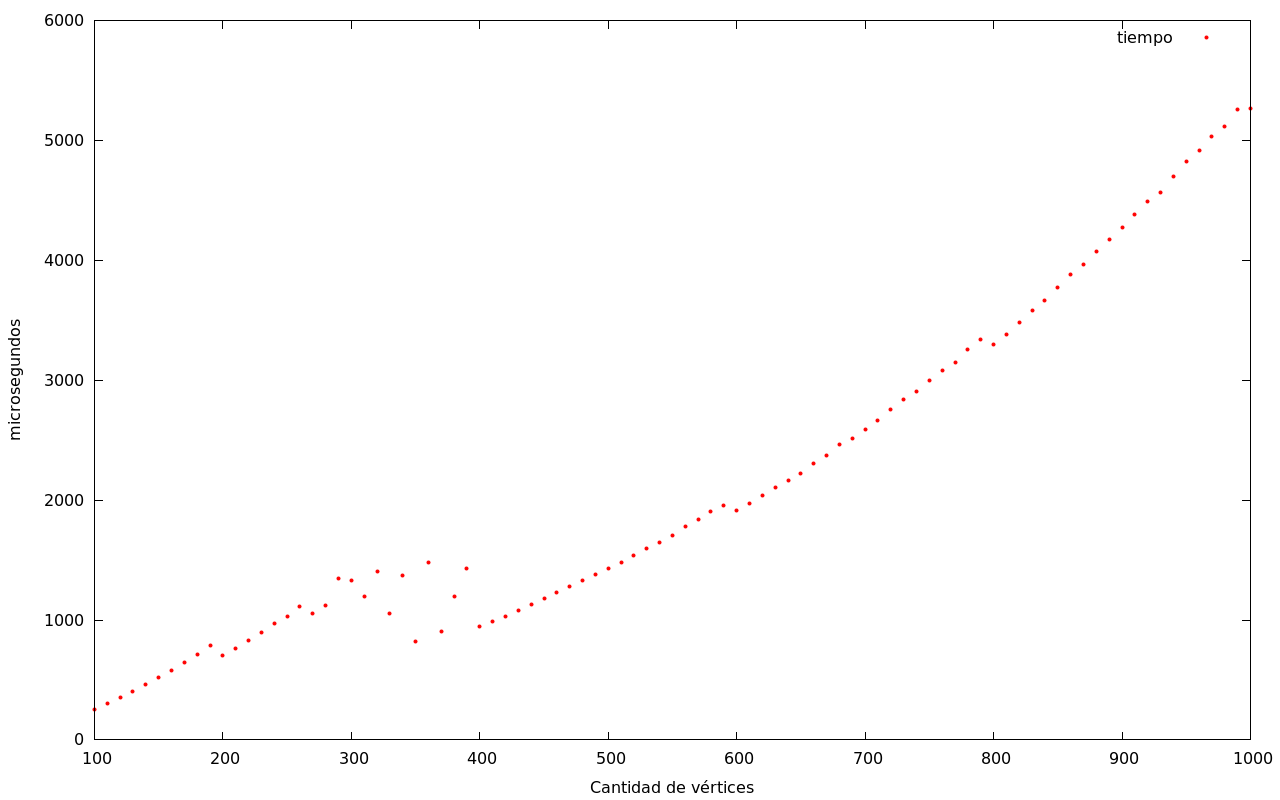
\includegraphics[scale=0.35]{imagenes/grafico-greedy-ac.png}
  \end{center}
\end{figure}

\vspace*{0.5cm}


\newpage
\subsubsection{Test 2 - algoritmo goloso, con aleatorización en las aritas}

(ver \verb|info.2.k.dat|) \medskip

En este test, tenemos $n$ nodos, con $n$ inicializado en 100, incrementándose de a 10 hasta alcanzar 1000, $m$ inicializado en 500, incremendtándose de a 50 hasta alcanzar 5000 (vale 5 veces $n$) y $k$ vale $\frac{n}{20}$.

Para cada instancia se toma el \textbf{valor mínimo} mediado en microsegundos luego de \textbf{10 corridas}.

Dada una combinación de $m$, $n$ y $k$, se generaron 5 instancias aleatorias con dicha combinación y se consideró el promedio entre ellas.

\vspace*{0.5cm}

\begin{figure}[h]
  \begin{center}
    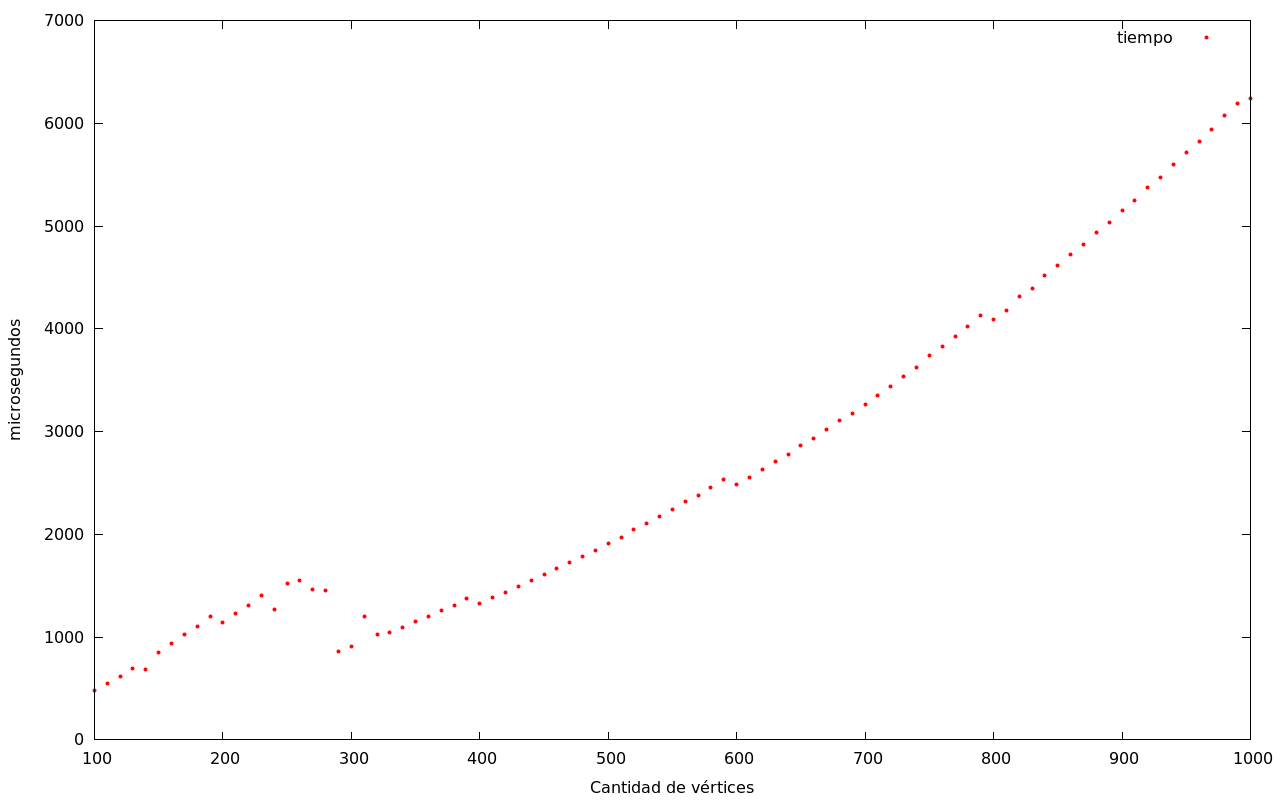
\includegraphics[scale=0.35]{imagenes/grafico-greedy-a.png}
  \end{center}
\end{figure}

\vspace{0.5cm}


\newpage
\subsubsection{Test 3 - algoritmo goloso, con aleatorización en conjuntos}

(ver \verb|info.2.k.dat|) \medskip

En este test, tenemos $n$ nodos, con $n$ inicializado en 100, incrementándose de a 10 hasta alcanzar 1000, $m$ inicializado en 500, incremendtándose de a 50 hasta alcanzar 5000 (vale 5 veces $n$) y $k$ vale $\frac{n}{20}$.

Para cada instancia se toma el \textbf{valor mínimo} mediado en microsegundos luego de \textbf{10 corridas}.

Dada una combinación de $m$, $n$ y $k$, se generaron 5 instancias aleatorias con dicha combinación y se consideró el promedio entre ellas.

\vspace*{0.5cm}

\begin{figure}[h]
  \begin{center}
    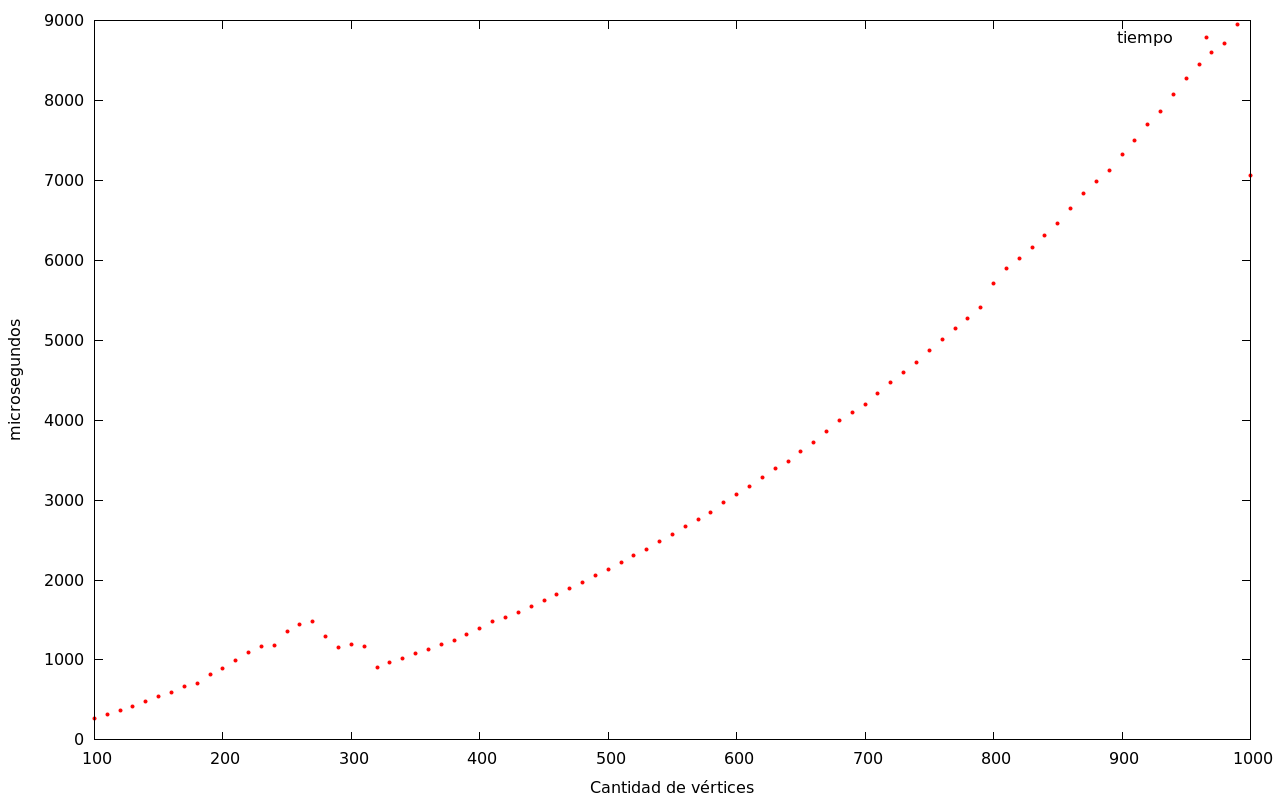
\includegraphics[scale=0.35]{imagenes/grafico-greedy-c.png}
  \end{center}
\end{figure}

\vspace{0.5cm}


\newpage
\subsubsection{Test 4 - algoritmo goloso, con aleatorización en aristas y conjuntos}

(ver \verb|info.2.k.dat|) \medskip

En este test, tenemos $n$ nodos, con $n$ inicializado en 100, incrementándose de a 10 hasta alcanzar 1000, $m$ inicializado en 500, incremendtándose de a 50 hasta alcanzar 5000 (vale 5 veces $n$) y $k$ vale $\frac{n}{20}$.

Para cada instancia se toma el \textbf{valor mínimo} mediado en microsegundos luego de \textbf{10 corridas}.

Dada una combinación de $m$, $n$ y $k$, se generaron 5 instancias aleatorias con dicha combinación y se consideró el promedio entre ellas.

\vspace*{0.5cm}

\begin{figure}[h]
  \begin{center}
    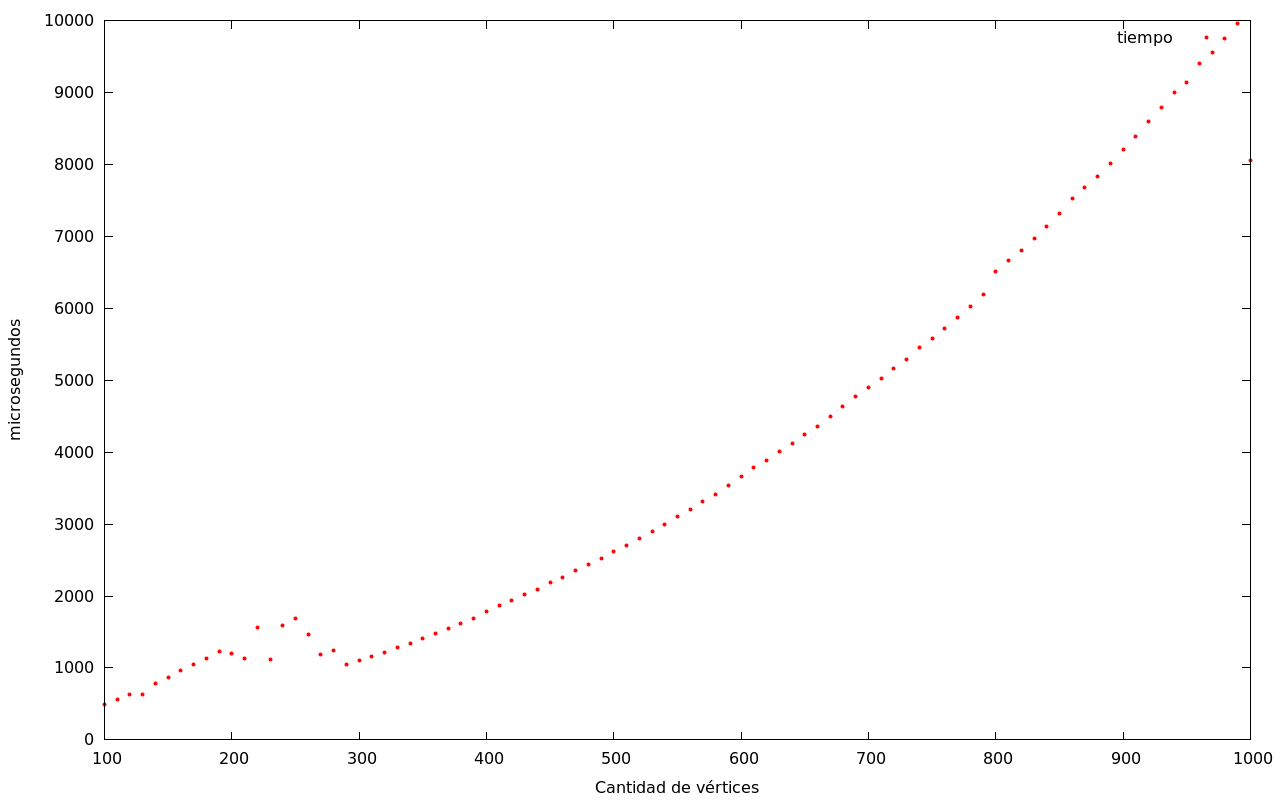
\includegraphics[scale=0.35]{imagenes/grafico-greedy.png}
  \end{center}
\end{figure}

\vspace{0.5cm}
